\documentclass[aspectratio=169,12pt]{beamer}

\usepackage[utf8]{inputenc}
\usepackage[T1]{fontenc}
\IfFileExists{spanish.ldf}{\usepackage[spanish]{babel}}{\usepackage{babel}\babelprovide[import,main]{spanish}}
\usepackage{helvet}
\usepackage{booktabs}
\usepackage{array}
\usepackage{tikz}
\usepackage{pgfpages}
\usetikzlibrary{arrows.meta,positioning,calc,fit,shapes.geometric}

\ifdefined\ModoNotas
  \setbeameroption{show notes on second screen=right}
\else
  \setbeameroption{hide notes}
\fi

% Cifras compartidas por la presentación.
% Fuente autoritativa: flujo de fondos corregido y el informe vigente.
\newcommand{\PresupuestoAnioUno}{USD~228.303,06}
\newcommand{\CapitalMinimo}{USD~228.303,06}
\newcommand{\VANBase}{USD~103.250,74}
\newcommand{\TIRBase}{36,83\%}
\newcommand{\TasaDescuento}{20\%}
\newcommand{\VANConservador}{USD~-223.190,04}
\newcommand{\VANRetencionBaja}{USD~-18.477,62}
\newcommand{\Dotacion}{4~FTE}
\newcommand{\CapacidadAnual}{7.680~h}
\newcommand{\DuracionDesarrollo}{12~meses}
\newcommand{\SprintsAnuales}{26}
\newcommand{\VentasDos}{300}
\newcommand{\VentasTres}{800}
\newcommand{\VentasCuatro}{1.680}
\newcommand{\PrecioKit}{USD~400}
\newcommand{\PrecioParche}{USD~25}
\newcommand{\CostoDirectoKit}{USD~102,46}
\newcommand{\CostoLogisticoKit}{USD~69,06}
\newcommand{\CostoDirectoParche}{USD~11,33}
\newcommand{\FlujoDos}{USD~15.968,37}
\newcommand{\FlujoTres}{USD~139.335,27}
\newcommand{\FlujoCuatro}{USD~451.017,53}
\newcommand{\MedicosDos}{18}
\newcommand{\MedicosTres}{35}
\newcommand{\MedicosCuatro}{56}
\newcommand{\ClinicasDos}{7}
\newcommand{\ClinicasTres}{15}
\newcommand{\ClinicasCuatro}{24}
\newcommand{\AutoresPresentacion}{%
  Marco Brischetto \quad Lautaro García Vitale\\
  Gabriel José Vigo Abad \quad Juan Ignacio Giachetti\\
  Ignacio E. Cavicchioli \quad Martina Monti\\
  Francisco Del Rio \quad Santiago Manuel Cabrera}


% Paleta compacta: azul FIUBA, turquesa y grises neutros.
\definecolor{fiuba}{HTML}{005A8D}
\definecolor{turquesa}{HTML}{00A6A6}
\definecolor{tinta}{HTML}{263746}
\definecolor{claro}{HTML}{F2F6F8}
\definecolor{medio}{HTML}{D8E4EA}
\definecolor{negativo}{HTML}{A64040}
\definecolor{positivo}{HTML}{247060}

\renewcommand{\familydefault}{\sfdefault}
\setbeamercolor{normal text}{fg=tinta,bg=white}
\setbeamercolor{structure}{fg=fiuba}
\setbeamercolor{frametitle}{fg=fiuba,bg=white}
\setbeamercolor{alerted text}{fg=turquesa}
\setbeamercolor{block title}{fg=white,bg=fiuba}
\setbeamercolor{block body}{fg=tinta,bg=claro}
\setbeamerfont{frametitle}{size=\fontsize{23}{26}\selectfont,series=\bfseries}
\setbeamerfont{normal text}{size=\fontsize{14}{18}\selectfont}
\setbeamerfont{block title}{series=\bfseries}
\setbeamertemplate{navigation symbols}{}
\setbeamertemplate{itemize item}{\color{turquesa}\raisebox{0.15ex}{\scriptsize$\blacktriangleright$}}
\setbeamertemplate{itemize subitem}{\color{turquesa}\scriptsize$\bullet$}
\setbeamertemplate{blocks}[rounded][shadow=false]
\setbeamersize{text margin left=0.6cm,text margin right=0.6cm}

\newcommand{\ExpositorActual}{1}
\newcommand{\speaker}[1]{\renewcommand{\ExpositorActual}{#1}}
\newif\ifrespaldo
\respaldofalse

\setbeamertemplate{footline}{%
  \leavevmode%
  \hbox{%
    \begin{beamercolorbox}[wd=.33\paperwidth,ht=3.2ex,dp=1.2ex,leftskip=.6cm]{author in head/foot}%
      \color{fiuba}\bfseries\ifrespaldo Respaldo\else Expositor \ExpositorActual\fi
    \end{beamercolorbox}%
    \begin{beamercolorbox}[wd=.47\paperwidth,ht=3.2ex,dp=1.2ex,center]{title in head/foot}%
      \color{tinta}TC024 - Gestión de proyectos
    \end{beamercolorbox}%
    \begin{beamercolorbox}[wd=.20\paperwidth,ht=3.2ex,dp=1.2ex,rightskip=.6cm plus1fil]{date in head/foot}%
      \color{fiuba}\bfseries\ifrespaldo A\insertframenumber\else\insertframenumber/16\fi
    \end{beamercolorbox}%
  }%
  \vskip0pt%
}

\setbeamertemplate{frametitle}{%
  \vspace{0.22cm}%
  \begin{beamercolorbox}[wd=\paperwidth,sep=0pt,leftskip=0.6cm]{frametitle}
    \insertframetitle\par
    \vspace{0.08cm}\color{turquesa}\rule{2.1cm}{1.4pt}
  \end{beamercolorbox}%
}

\newcommand{\fuente}[1]{\vfill\hfill{\color{tinta!68}\fontsize{7.3}{8.5}\selectfont Fuente: #1}}
\newcommand{\pill}[1]{\tikz[baseline=(X.base)]\node[rounded corners=7pt,fill=turquesa!12,draw=turquesa!55,inner xsep=8pt,inner ysep=3pt,font=\bfseries\small] (X) {#1};}
\newcommand{\bigmetric}[3]{%
  \begin{beamercolorbox}[wd=\linewidth,sep=0.20cm,center,rounded=true]{block body}
    {\color{#1}\fontsize{22}{24}\selectfont\bfseries #2}\par
    \vspace{0.04cm}{\fontsize{9.5}{11}\selectfont #3}
  \end{beamercolorbox}}
\newcommand{\notatiempo}[4]{%
  \note{%
    \textbf{Tiempo objetivo:} #1\par\medskip
    \textbf{Objetivo:} #2\par\medskip
    #3\par\medskip
    \textbf{Transición:} #4}}

\title{Sistema inteligente multimodal de detección y predicción de glucosa}
\subtitle{Plan técnico, operativo y financiero para un MVP en doce meses}
\author{Grupo 3}
\institute{Facultad de Ingeniería - Universidad de Buenos Aires}
\date{TC024 - Gestión de proyectos}

\begin{document}

% -----------------------------------------------------------------------------
% Expositor 1
% -----------------------------------------------------------------------------
\speaker{1}
\begin{frame}
  \begin{columns}[c,onlytextwidth]
    \begin{column}{0.77\textwidth}
      {\color{fiuba}\fontsize{27}{31}\selectfont\bfseries Sistema inteligente multimodal de detección y predicción de glucosa\par}
      \vspace{0.35cm}
      {\color{turquesa}\fontsize{16}{19}\selectfont Un MVP trazable para aportar contexto al seguimiento metabólico\par}
      \vspace{0.48cm}
      {\fontsize{10.3}{13}\selectfont\AutoresPresentacion\par}
      \vspace{0.38cm}
      \pill{Grupo 3}\hspace{0.16cm}\pill{TC024}\hspace{0.16cm}\pill{30 minutos}
    \end{column}
    \begin{column}{0.20\textwidth}
      \centering
      \IfFileExists{../Gestion de proyectos practica/logo-fiuba.png}{%
        
\includegraphics[width=\linewidth]{../Gestion de proyectos practica/logo-fiuba.png}%
      }{%
        {\color{fiuba}\fontsize{28}{32}\selectfont\bfseries FIUBA}%
      }
    \end{column}
  \end{columns}
  \notatiempo{1:20}{Presentar el proyecto y anticipar la tesis de la exposición.}{
    El trabajo no parte de la promesa de un producto clínicamente validado. Parte de un problema de seguimiento y propone un plan verificable para llegar a un MVP funcional y técnico en doce meses. Nombrar al equipo como Grupo 3 y aclarar que las ocho personas participarán en bloques consecutivos.}{
    Para entender la propuesta, primero hay que separar dos necesidades: medir una variación y poder interpretarla.}
\end{frame}

\begin{frame}{La brecha: medir no siempre alcanza para interpretar}
  \begin{columns}[T,onlytextwidth]
    \begin{column}{0.31\textwidth}
      \begin{block}{1. La señal}
        Los CGM muestran niveles, tendencias y alertas de glucosa.
      \end{block}
    \end{column}
    \begin{column}{0.31\textwidth}
      \begin{block}{2. El contexto}
        Alimentación, estrés y actividad suelen quedar en registros separados.
      \end{block}
    \end{column}
    \begin{column}{0.31\textwidth}
      \begin{block}{3. La interpretación}
        Relacionar ambas fuentes exige evidencia y evaluación profesional.
      \end{block}
    \end{column}
  \end{columns}
  \vspace{0.34cm}
  \begin{beamercolorbox}[sep=0.28cm,rounded=true,center]{block body}
    {\color{fiuba}\bfseries\fontsize{22}{25}\selectfont $\approx$4 millones}\par
    {\large adultos con diabetes tipo 2 como referencia poblacional en Argentina}\par
    {\small No equivale al mercado accesible ni a demanda confirmada.}
  \end{beamercolorbox}
  \fuente{IDF Diabetes Atlas 2025 e informe del proyecto.}
  \notatiempo{2:10}{Definir el problema sin exagerar el beneficio esperado.}{
    Explicar que el seguimiento actual puede mostrar qué ocurrió, pero la relación con hábitos y señales fisiológicas suele quedar dispersa. La cifra poblacional solo da escala: no debe presentarse como cantidad de clientes. La oportunidad está en investigar si una integración multimodal puede aportar contexto de manera útil.}{
    El siguiente bloque presenta qué propone exactamente el proyecto y, con igual importancia, qué no promete.}
\end{frame}

% -----------------------------------------------------------------------------
% Expositor 2
% -----------------------------------------------------------------------------
\speaker{2}
\begin{frame}{La propuesta: contexto multimodal, no diagnóstico}
  \begin{center}
  \begin{tikzpicture}[node distance=0.55cm and 0.65cm,
    box/.style={rounded corners=5pt,draw=fiuba!60,fill=claro,minimum width=3.15cm,minimum height=1.45cm,align=center,font=\bfseries},
    out/.style={rounded corners=5pt,draw=turquesa,fill=turquesa!10,minimum width=3.5cm,minimum height=1.45cm,align=center,font=\bfseries},
    arr/.style={-{Stealth[length=3mm]},line width=1.1pt,draw=fiuba}]
    \node[box] (sudor) {Biomarcadores\\en sudor};
    \node[box,right=of sudor] (fisiologia) {Señales\\fisiológicas};
    \node[box,right=of fisiologia] (historial) {Historial\\y contexto};
    \node[out,below=0.8cm of fisiologia] (salida) {Factores probablemente asociados\\+ estimaciones con incertidumbre};
    \draw[arr] (sudor.south) |- (salida.west);
    \draw[arr] (fisiologia) -- (salida);
    \draw[arr] (historial.south) |- (salida.east);
  \end{tikzpicture}
  \end{center}
  \vspace{0.25cm}
  \begin{columns}[T,onlytextwidth]
    \begin{column}{0.49\textwidth}
      \textbf{Misión}\par
      Integrar mediciones y contexto para facilitar el seguimiento metabólico.
    \end{column}
    \begin{column}{0.49\textwidth}
      \textbf{Límite explícito}\par
      No establece causalidad ni emite recomendaciones automáticas de tratamiento.
    \end{column}
  \end{columns}
  \fuente{Definición, misión y visión del informe.}
  \notatiempo{1:40}{Exponer la propuesta de valor y su límite clínico.}{
    Presentar la integración de tres fuentes: biomarcadores, señales fisiológicas e historial. Las salidas son asociaciones y estimaciones que deberán informar incertidumbre. Repetir que el sistema complementa a los CGM y que la interpretación final no se convierte en diagnóstico o tratamiento automático.}{
    Esa misión se concreta en un resultado mensurable: un MVP compuesto por cuatro partes.}
\end{frame}

\begin{frame}{Qué entregamos: un MVP de cuatro componentes}
  \begin{columns}[T,onlytextwidth]
    \begin{column}{0.49\textwidth}
      \begin{block}{Parche descartable}
        Glucosa, lactato, cortisol y pH en sudor. Objetivo de recambio: 7 días.
      \end{block}
      \begin{block}{Lector reutilizable}
        Lectura óptica y electroquímica, procesamiento, memoria y BLE.
      \end{block}
    \end{column}
    \begin{column}{0.49\textwidth}
      \begin{block}{Pulsera reutilizable}
        Frecuencia cardíaca, actividad y temperatura de piel.
      \end{block}
      \begin{block}{Aplicación móvil}
        Sincronización, historial, análisis, avisos e incertidumbre.
      \end{block}
    \end{column}
  \end{columns}
  \vspace{0.18cm}
  \begin{beamercolorbox}[sep=0.20cm,rounded=true,center]{block body}
    \textbf{Objetivo SMART:} MVP integrado y aceptado funcional y técnicamente al mes 12.
  \end{beamercolorbox}
  \fuente{Objetivo y entregables mensurables del informe.}
  \notatiempo{1:50}{Definir con precisión el resultado del proyecto.}{
    Describir las cuatro piezas y remarcar la separación entre consumible y elementos reutilizables. El criterio de éxito no es fabricar un producto comercial: es aceptar un MVP con pruebas, limitaciones y documentación. La validación clínica y la certificación comercial quedan fuera de estos doce meses.}{
    Con el alcance definido, el siguiente expositor muestra cómo circula la información entre los componentes.}
\end{frame}

% -----------------------------------------------------------------------------
% Expositor 3
% -----------------------------------------------------------------------------
\speaker{3}
\begin{frame}{Cómo fluye la información}
  \centering
  \begin{tikzpicture}[node distance=0.55cm and 0.75cm,
    dev/.style={rounded corners=5pt,draw=fiuba!65,fill=claro,minimum width=3.3cm,minimum height=1.45cm,align=center},
    app/.style={rounded corners=5pt,draw=turquesa,fill=turquesa!12,minimum width=3.45cm,minimum height=1.6cm,align=center,font=\bfseries},
    out/.style={rounded corners=5pt,draw=fiuba,fill=white,minimum width=3.4cm,minimum height=1.3cm,align=center},
    arr/.style={-{Stealth[length=3mm]},line width=1.15pt,draw=fiuba},
    optional/.style={{Stealth[length=3mm]}-{Stealth[length=3mm]},dashed,line width=1pt,draw=turquesa}]
    \node[dev] (brazo) {\textbf{Brazo}\\parche + lector};
    \node[dev,below=0.65cm of brazo] (pulsera) {\textbf{Muñeca}\\pulsera};
    \node[app,right=1.4cm of $(brazo)!0.5!(pulsera)$] (telefono) {Aplicación móvil\\hub de datos};
    \node[dev,right=1.05cm of telefono] (nube) {Servicio remoto\\alternativa a evaluar};
    \node[out,below=0.75cm of telefono] (resultados) {Historial, estimaciones,\\incertidumbre y avisos};
    \draw[arr] (brazo.east) -- node[above,sloped,font=\small]{BLE} (telefono.west |- brazo.east);
    \draw[arr] (pulsera.east) -- node[below,sloped,font=\small]{BLE} (telefono.west |- pulsera.east);
    \draw[optional] (telefono) -- node[above,font=\small]{Internet} (nube);
    \draw[arr] (telefono) -- (resultados);
  \end{tikzpicture}
  \vspace{0.3cm}
  \begin{columns}[c,onlytextwidth]
    \begin{column}{0.32\textwidth}\centering\pill{Sincronización: 5 min}\end{column}
    \begin{column}{0.32\textwidth}\centering\pill{Buffer local: 24 h}\end{column}
    \begin{column}{0.32\textwidth}\centering\pill{IA local o remota}\end{column}
  \end{columns}
  \fuente{Arquitectura preliminar del informe.}
  \notatiempo{1:45}{Explicar el recorrido de los datos y las decisiones aún abiertas.}{
    El lector y la pulsera se comunican solo con el teléfono. Ante una pérdida de BLE, cada dispositivo conserva hasta 24 horas y reenvía el bloque al reconectarse. La ejecución de los modelos podrá ser local o remota; el proyecto no compromete ambas alternativas y deberá elegir una según costo, privacidad, conectividad y capacidad de cómputo.}{
    Para sostener este flujo, cada componente tiene funciones y pruebas propias.}
\end{frame}

\begin{frame}{Qué mide y qué verifica cada componente}
  \begin{columns}[T,onlytextwidth]
    \begin{column}{0.24\textwidth}
      \begin{block}{Parche}
        \small Color, señal electroquímica, adhesión, reactivos e interferencias.
      \end{block}
    \end{column}
    \begin{column}{0.24\textwidth}
      \begin{block}{Lector}
        \small Óptica, potenciostato, batería, memoria, BLE y acople.
      \end{block}
    \end{column}
    \begin{column}{0.24\textwidth}
      \begin{block}{Pulsera}
        \small PPG, IMU, temperatura, batería, memoria y BLE.
      \end{block}
    \end{column}
    \begin{column}{0.24\textwidth}
      \begin{block}{Aplicación}
        \small Vinculación, historial, faltantes, modelos, incertidumbre y ayuda.
      \end{block}
    \end{column}
  \end{columns}
  \vspace{0.38cm}
  \begin{beamercolorbox}[sep=0.28cm,rounded=true]{block body}
    \centering
    \textbf{Trazabilidad extremo a extremo}\par
    requisito $\rightarrow$ protocolo $\rightarrow$ resultado $\rightarrow$ desvío $\rightarrow$ decisión
  \end{beamercolorbox}
  \vspace{0.25cm}
  \centering\large La integración no se considera demostrada hasta probar el sistema completo.
  \fuente{Requerimientos y diseño preliminar del informe.}
  \notatiempo{1:45}{Mostrar que el proyecto no reduce la factibilidad a una lista de componentes.}{
    Cada objeto requiere pruebas propias, pero la aceptación depende del recorrido completo. La trazabilidad conecta cada requisito con una evidencia; si una prueba falla, el desvío debe quedar registrado y producir una decisión. Evitar decir que los sensores ya alcanzan desempeño clínico: son elementos de una arquitectura a verificar.}{
    El siguiente bloque resume las hipótesis técnicas cuantificadas y cómo se transforman en criterios de aceptación.}
\end{frame}

% -----------------------------------------------------------------------------
% Expositor 4
% -----------------------------------------------------------------------------
\speaker{4}
\begin{frame}{Factibilidad técnica: objetivos verificables}
  \begin{columns}[T,onlytextwidth]
    \begin{column}{0.235\textwidth}\bigmetric{fiuba}{7 días}{autonomía objetivo}\end{column}
    \begin{column}{0.235\textwidth}\bigmetric{fiuba}{128 KiB}{memoria utilizable mínima}\end{column}
    \begin{column}{0.235\textwidth}\bigmetric{turquesa}{24 h}{datos locales por dispositivo}\end{column}
    \begin{column}{0.235\textwidth}\bigmetric{turquesa}{5 min}{sincronización nominal}\end{column}
  \end{columns}
  \vspace{0.42cm}
  \begin{columns}[T,onlytextwidth]
    \begin{column}{0.49\textwidth}
      \textbf{Ensayos de ingeniería}
      \begin{itemize}
        \item corriente por estado y descarga completa;
        \item llenado, apagado y recuperación del buffer;
        \item pérdida y reconexión BLE.
      \end{itemize}
    \end{column}
    \begin{column}{0.49\textwidth}
      \textbf{Ensayos de sensado}
      \begin{itemize}
        \item rango, repetibilidad e interferencias;
        \item calibración y estabilidad de reactivos;
        \item referencia para cada salida.
      \end{itemize}
    \end{column}
  \end{columns}
  \fuente{Dimensionamiento preliminar del informe; valores sujetos a ensayo.}
  \notatiempo{1:50}{Distinguir cálculo preliminar de resultado demostrado.}{
    Los cuatro números son especificaciones de diseño. La autonomía se estimó con baterías de 750 y 850 mAh, consumos medios máximos de 3,5 y 4 mA y 20 por ciento de reserva. La memoria parte de registros de 64 bytes cada dos minutos. La aceptación exige reemplazar estos cálculos por mediciones y ensayos completos.}{
    La factibilidad se aprende por etapas: primero subsistemas, luego prototipo integrado y finalmente MVP.}
\end{frame}

\begin{frame}{Del prototipo al MVP aceptado}
  \centering
  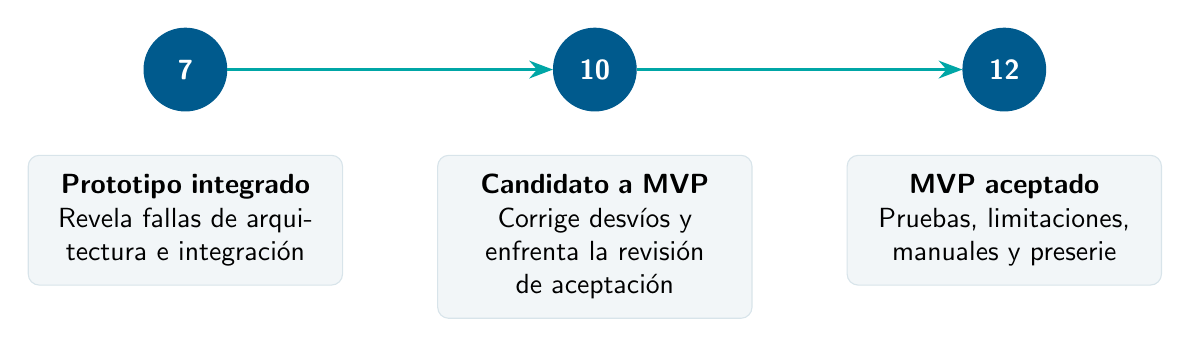
\begin{tikzpicture}[x=1cm,y=1cm,
    milestone/.style={circle,minimum size=1.05cm,draw=fiuba,fill=fiuba,text=white,font=\bfseries},
    labelbox/.style={rounded corners=4pt,draw=medio,fill=claro,text width=3.5cm,align=center,inner sep=7pt},
    arr/.style={-{Stealth[length=3mm]},line width=1.2pt,draw=turquesa}]
    \node[milestone] (m7) at (0,1.2) {7};
    \node[milestone] (m10) at (5.2,1.2) {10};
    \node[milestone] (m12) at (10.4,1.2) {12};
    \draw[arr] (m7) -- (m10);
    \draw[arr] (m10) -- (m12);
    \node[labelbox,below=0.55cm of m7] {\textbf{Prototipo integrado}\\Revela fallas de arquitectura e integración};
    \node[labelbox,below=0.55cm of m10] {\textbf{Candidato a MVP}\\Corrige desvíos y enfrenta la revisión de aceptación};
    \node[labelbox,below=0.55cm of m12] {\textbf{MVP aceptado}\\Pruebas, limitaciones, manuales y preserie};
  \end{tikzpicture}
  \vspace{0.32cm}
  \begin{beamercolorbox}[sep=0.22cm,rounded=true,center]{block body}
    El prototipo es un instrumento de aprendizaje; no es el producto final ni validación clínica.
  \end{beamercolorbox}
  \fuente{Plan de producto y criterios de aceptación del informe.}
  \notatiempo{1:40}{Evitar la confusión central entre prototipo y resultado final.}{
    En el mes 7 se busca descubrir fallas cuando todavía hay tiempo de corregirlas. El mes 10 congela un candidato que enfrenta una revisión formal. El mes 12 entrega el MVP aceptado, con limitaciones y documentación. La validación clínica y la certificación comercial requerirían otra etapa, presupuesto y autoridades competentes.}{
    El quinto bloque muestra cómo el cronograma reserva tiempo y recursos para recorrer esas etapas.}
\end{frame}

% -----------------------------------------------------------------------------
% Expositor 5
% -----------------------------------------------------------------------------
\speaker{5}
\begin{frame}{Plan de 12 meses: reducir riesgo por etapas}
  \centering
  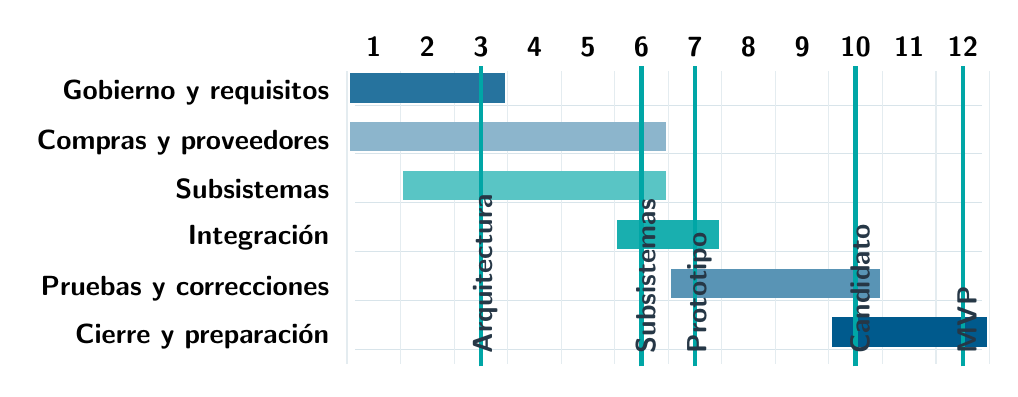
\begin{tikzpicture}[x=0.68cm,y=0.62cm,font=\fontsize{7.8}{9}\selectfont]
    \foreach \m in {1,...,12}{\node[font=\bfseries] at (\m,7.2) {\m};}
    \foreach \y in {1,...,6}{\draw[medio] (0.65,\y) -- (12.35,\y);}
    \foreach \m in {1,...,13}{\draw[medio!70] (\m-0.5,0.7) -- (\m-0.5,6.7);}
    \node[anchor=e,font=\bfseries] at (0.35,6.35) {Gobierno y requisitos};
    \node[anchor=e,font=\bfseries] at (0.35,5.35) {Compras y proveedores};
    \node[anchor=e,font=\bfseries] at (0.35,4.35) {Subsistemas};
    \node[anchor=e,font=\bfseries] at (0.35,3.35) {Integración};
    \node[anchor=e,font=\bfseries] at (0.35,2.35) {Pruebas y correcciones};
    \node[anchor=e,font=\bfseries] at (0.35,1.35) {Cierre y preparación};
    \fill[fiuba!85] (0.55,6.05) rectangle (3.45,6.65);
    \fill[fiuba!45] (0.55,5.05) rectangle (6.45,5.65);
    \fill[turquesa!65] (1.55,4.05) rectangle (6.45,4.65);
    \fill[turquesa!90] (5.55,3.05) rectangle (7.45,3.65);
    \fill[fiuba!65] (6.55,2.05) rectangle (10.45,2.65);
    \fill[fiuba] (9.55,1.05) rectangle (12.45,1.65);
    \foreach \x/\lab in {3/Arquitectura,6/Subsistemas,7/Prototipo,10/Candidato,12/MVP}{%
      \draw[turquesa,line width=1.6pt] (\x,0.65) -- (\x,6.8);
      \node[rotate=90,anchor=west,color=tinta,font=\bfseries] at (\x+0.08,0.72) {\lab};}
  \end{tikzpicture}
  \vspace{0.15cm}
  \small Dependencias externas en el Gantt; desarrollo e iteración técnica en sprints.
  \fuente{Cronograma maestro resumido y plan detallado del Excel.}
  \notatiempo{1:50}{Explicar la secuencia y las dependencias críticas.}{
    La arquitectura habilita compras y protocolos. Los subsistemas deben producir evidencia antes de la integración. Las compras, importación y laboratorios atraviesan varios meses porque dependen de terceros. La preparación comercial comienza en los meses 9 a 12, pero no hay ventas ni demostradores durante el año 1.}{
    El cronograma se sostiene con una dotación anual y una metodología híbrida.}
\end{frame}

\begin{frame}{Cómo trabajaremos: dotación anual y método híbrido}
  \begin{columns}[T,onlytextwidth]
    \begin{column}{0.34\textwidth}
      \bigmetric{fiuba}{\Dotacion}{dos perfiles de ingeniería + dos técnicos/administrativos}
      \vspace{0.22cm}
      \bigmetric{turquesa}{\CapacidadAnual}{capacidad bruta de control, no base del presupuesto}
    \end{column}
    \begin{column}{0.63\textwidth}
      \begin{block}{Gantt maestro}
        Compras, proveedores, importación, laboratorios, preserie y revisiones.
      \end{block}
      \begin{block}{\SprintsAnuales{} sprints quincenales}
        Electrónica, firmware, aplicación, modelos, documentación y correcciones.
      \end{block}
      \begin{block}{Gobierno mensual}
        Alcance, costo, riesgos, inventario, evidencia y decisiones de hito.
      \end{block}
    \end{column}
  \end{columns}
  \fuente{Organización y metodología de trabajo del informe.}
  \notatiempo{1:40}{Justificar por qué se presupuestan personas y no una bolsa de horas.}{
    El compromiso es contar con cuatro personas full-time durante doce meses. Las 7.680 horas sirven para controlar capacidad y carga; no se pagan además como horas valorizadas. El Gantt gobierna plazos externos y los sprints absorben aprendizaje técnico. Cada historia termina con responsable, criterio de aceptación y evidencia.}{
    Incluso con este esquema, el proyecto conserva riesgos altos que deben gestionarse explícitamente.}
\end{frame}

% -----------------------------------------------------------------------------
% Expositor 6
% -----------------------------------------------------------------------------
\speaker{6}
\begin{frame}{Riesgos dominantes y respuesta prevista}
  \begin{columns}[T,onlytextwidth]
    \begin{column}{0.46\textwidth}
      \centering\textbf{RPN preliminar}\par\vspace{0.12cm}
      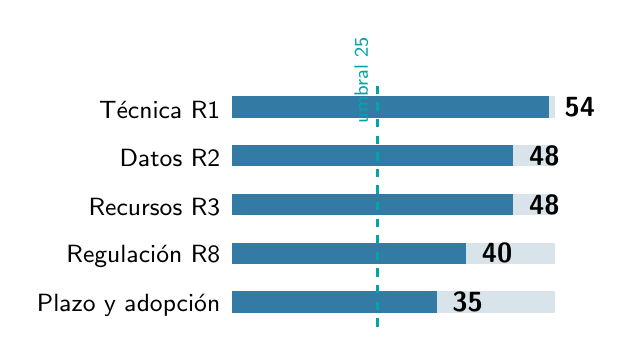
\begin{tikzpicture}[x=0.075cm,y=0.62cm,font=\small]
        \foreach \y/\name/\val in {5/Técnica R1/54,4/Datos R2/48,3/Recursos R3/48,2/Regulación R8/40,1/Plazo y adopción/35}{%
          \node[anchor=e] at (0,\y) {\name};
          \fill[medio] (0.4,\y-0.22) rectangle (55,\y+0.22);
          \fill[fiuba!80] (0.4,\y-0.22) rectangle (\val,\y+0.22);
          \node[anchor=west,font=\bfseries] at (\val+1,\y) {\val};}
        \draw[turquesa,dashed,line width=1.1pt] (25,0.5) -- (25,5.5);
        \node[rotate=90,anchor=south,color=turquesa,font=\scriptsize] at (25,5.55) {umbral 25};
      \end{tikzpicture}
    \end{column}
    \begin{column}{0.51\textwidth}
      \begin{block}{Reducir incertidumbre}
        Prototipos, ensayos, fuentes de datos y revisión especializada.
      \end{block}
      \begin{block}{Proteger el plan}
        Alternativas de proveedor, hitos, control de alcance y reserva técnica trazable.
      \end{block}
      \begin{block}{No ocultar límites}
        Un riesgo residual alto permanece abierto y documentado.
      \end{block}
    \end{column}
  \end{columns}
  \fuente{Matriz de riesgos del informe; escala severidad por ocurrencia.}
  \notatiempo{1:50}{Presentar los riesgos como información para decidir, no como una formalidad.}{
    La integración y calibración es el riesgo principal. También son críticos los datos para IA, los recursos especializados y la definición regulatoria. El umbral de 25 obliga a mitigar y revisar. La severidad de algunos riesgos no baja: se intenta reducir su ocurrencia mediante evidencia, alternativas y decisiones tempranas.}{
    La incertidumbre no es solo técnica: el canal comercial también debe ser validado con un embudo concreto.}
\end{frame}

\begin{frame}{Llegada al mercado: médicos como canal principal}
  \begin{columns}[T,onlytextwidth]
    \begin{column}{0.32\textwidth}
      \begin{block}{Año 2}
        \centering
        \textbf{125} prospectos\par
        $\downarrow$\par
        \textbf{25} aliados\par
        \MedicosDos{} médicos + \ClinicasDos{} clínicas\par
        $\downarrow$\par
        {\color{fiuba}\bfseries\Large \VentasDos{} kits}
      \end{block}
    \end{column}
    \begin{column}{0.32\textwidth}
      \begin{block}{Año 3}
        \centering
        \textbf{250} prospectos\par
        $\downarrow$\par
        \textbf{50} aliados\par
        \MedicosTres{} médicos + \ClinicasTres{} clínicas\par
        $\downarrow$\par
        {\color{fiuba}\bfseries\Large \VentasTres{} kits}
      \end{block}
    \end{column}
    \begin{column}{0.32\textwidth}
      \begin{block}{Año 4}
        \centering
        \textbf{400} prospectos\par
        $\downarrow$\par
        \textbf{80} aliados\par
        \MedicosCuatro{} médicos + \ClinicasCuatro{} clínicas\par
        $\downarrow$\par
        {\color{fiuba}\bfseries\Large \VentasCuatro{} kits}
      \end{block}
    \end{column}
  \end{columns}
  \vspace{0.25cm}
  \centering\small Las clínicas concentran demostraciones y acuerdos; no se pagan derivaciones clínicas.
  \fuente{Embudo comercial base del informe y del Excel.}
  \notatiempo{1:40}{Mostrar cómo se obtienen las ventas sin partir de una cifra arbitraria.}{
    Cada año parte de prospectos calificados, una conversión del 20 por ciento y una cantidad explícita de médicos y clínicas aliados. Los kits vendidos surgen de pacientes alcanzables por aliado y adopción. Los médicos son el canal principal; las clínicas reciben un demostrador y onboarding. El embudo debe contrastarse antes de escalar.}{
    El siguiente bloque traduce el alcance, la producción y el canal en costos, precios y retorno.}
\end{frame}

% -----------------------------------------------------------------------------
% Expositor 7
% -----------------------------------------------------------------------------
\speaker{7}
\begin{frame}{Economía del proyecto: inversión y unidad productiva}
  \begin{columns}[T,onlytextwidth]
    \begin{column}{0.34\textwidth}
      \bigmetric{fiuba}{\PresupuestoAnioUno}{desarrollo, equipo, ensayos, preserie y reserva}
      \vspace{0.25cm}
      \begin{beamercolorbox}[sep=0.20cm,rounded=true,center]{block body}
        \textbf{Año 1}\par
        desarrollo e inversión\par
        \alert{sin ventas}
      \end{beamercolorbox}
    \end{column}
    \begin{column}{0.63\textwidth}
      \begin{block}{Kit reutilizable + primer parche}
        \begin{tabular}{@{}lr@{}}
          Precio de planificación & \textbf{\PrecioKit}\
          Fabricación directa & \CostoDirectoKit\
          Logística e importación & \CostoLogisticoKit\
        \end{tabular}
      \end{block}
      \begin{block}{Parche de recambio}
        \begin{tabular}{@{}lr@{}}
          Precio de planificación & \textbf{\PrecioParche}\
          Costo directo & \CostoDirectoParche\
        \end{tabular}
      \end{block}
      {\small Los costos productivos no incluyen por sí solos comisión, soporte ni estructura comercial.}
    \end{column}
  \end{columns}
  \fuente{Costeo trazable y presupuesto conciliado del informe y del Excel.}
  \notatiempo{1:50}{Explicar el orden de magnitud de la inversión y evitar interpretar el costo directo como margen neto.}{
    El año 1 requiere 228.303,06 dólares y no registra ventas. El costo directo del kit se construye con materiales, armado, programación, prueba y trazabilidad; la importación aplica una previsión académica del 45 por ciento sobre CIF, más partidas separadas. El precio de 400 dólares y el parche de 25 son supuestos de planificación a validar.}{
    Con estos supuestos, el flujo base resulta favorable, pero la sensibilidad cambia la conclusión.}
\end{frame}

\begin{frame}{Viabilidad: retorno favorable, sensibilidad alta}
  \begin{columns}[T,onlytextwidth]
    \begin{column}{0.31\textwidth}\bigmetric{positivo}{\VANBase}{VAN a una tasa anual de \TasaDescuento}\end{column}
    \begin{column}{0.31\textwidth}\bigmetric{positivo}{\TIRBase}{TIR anual del escenario base}\end{column}
    \begin{column}{0.31\textwidth}\bigmetric{fiuba}{\CapitalMinimo}{máximo déficit antes del financiamiento}\end{column}
  \end{columns}
  \vspace{0.30cm}
  \begin{columns}[T,onlytextwidth]
    \begin{column}{0.55\textwidth}
      \centering\textbf{Flujo anual sin financiamiento}\par\vspace{0.08cm}
      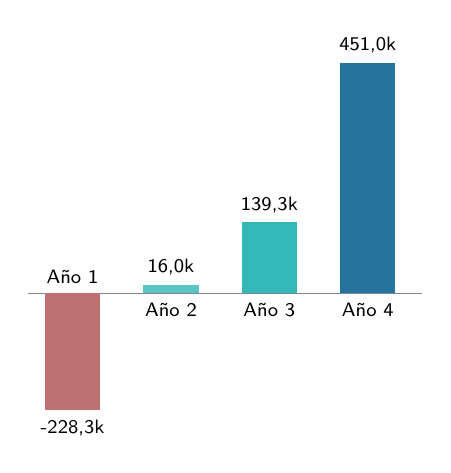
\begin{tikzpicture}[x=1.25cm,y=0.0065cm,font=\fontsize{7.5}{9}\selectfont]
        \draw[tinta!60] (-0.45,0) -- (3.55,0);
        \fill[negativo!75] (-0.28,-228) rectangle (0.28,0);
        \fill[turquesa!65] (0.72,0) rectangle (1.28,16);
        \fill[turquesa!80] (1.72,0) rectangle (2.28,139);
        \fill[fiuba!85] (2.72,0) rectangle (3.28,451);
        \node[above] at (0,0) {Año 1}; \node[below] at (0,-228) {-228,3k};
        \node[below] at (1,0) {Año 2}; \node[above] at (1,16) {16,0k};
        \node[below] at (2,0) {Año 3}; \node[above] at (2,139) {139,3k};
        \node[below] at (3,0) {Año 4}; \node[above] at (3,451) {451,0k};
      \end{tikzpicture}
    \end{column}
    \begin{column}{0.42\textwidth}
      \begin{beamercolorbox}[sep=0.18cm,rounded=true]{block body}
        \textbf{Escenario conservador}\par
        {\color{negativo}\bfseries \VANConservador}
      \end{beamercolorbox}
      \vspace{0.15cm}
      \begin{beamercolorbox}[sep=0.18cm,rounded=true]{block body}
        \textbf{Retención mensual 85\%}\par
        {\color{negativo}\bfseries \VANRetencionBaja}
      \end{beamercolorbox}
    \end{column}
  \end{columns}
  \fuente{Flujo de fondos corregido; valores en USD constantes.}
  \notatiempo{1:45}{Comunicar el resultado financiero con sus condiciones.}{
    El VAN base es positivo y la TIR supera la tasa de descuento, pero esto no garantiza viabilidad. El escenario conservador y una menor retención vuelven negativo el VAN. La decisión de escalar depende de validar el embudo, el costo unitario, la continuidad de recambios y la carga real de importación.}{
    Por eso el cierre no es una recomendación de lanzar sin condiciones, sino una secuencia de validaciones antes de escalar.}
\end{frame}

% -----------------------------------------------------------------------------
% Expositor 8
% -----------------------------------------------------------------------------
\speaker{8}
\begin{frame}{Qué hay que demostrar antes de escalar}
  \begin{center}
  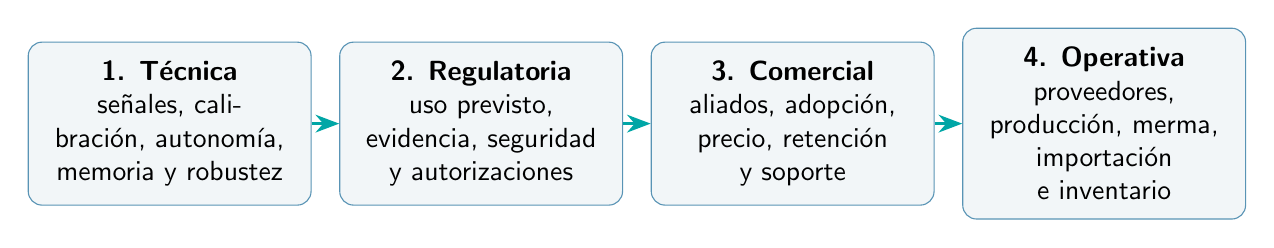
\begin{tikzpicture}[node distance=0.35cm,
    gate/.style={rounded corners=5pt,draw=fiuba!65,fill=claro,text width=3.1cm,minimum height=2.05cm,align=center,inner sep=7pt},
    arr/.style={-{Stealth[length=3mm]},line width=1.1pt,draw=turquesa}]
    \node[gate] (tec) {\textbf{1. Técnica}\\señales, calibración, autonomía, memoria y robustez};
    \node[gate,right=of tec] (reg) {\textbf{2. Regulatoria}\\uso previsto, evidencia, seguridad y autorizaciones};
    \node[gate,right=of reg] (com) {\textbf{3. Comercial}\\aliados, adopción, precio, retención y soporte};
    \node[gate,right=of com] (op) {\textbf{4. Operativa}\\proveedores, producción, merma, importación e inventario};
    \draw[arr] (tec) -- (reg);
    \draw[arr] (reg) -- (com);
    \draw[arr] (com) -- (op);
  \end{tikzpicture}
  \end{center}
  \vspace{0.38cm}
  \begin{beamercolorbox}[sep=0.25cm,rounded=true,center]{block body}
    \large Escalar solo cuando la evidencia sostenga simultáneamente el producto, el canal y la operación.
  \end{beamercolorbox}
  \fuente{Síntesis de factibilidad, riesgos y viabilidad del informe.}
  \notatiempo{1:45}{Transformar la incertidumbre en criterios de decisión.}{
    Las cuatro puertas se condicionan entre sí. Un prototipo técnicamente prometedor no alcanza si el uso previsto exige otra evidencia, si el canal no convierte o si la producción no puede sostenerse. Cada puerta tiene métricas, responsables y revisiones. La salida responsable también puede ser limitar alcance o documentar inviabilidad.}{
    La última diapositiva resume el compromiso concreto del proyecto.}
\end{frame}

\begin{frame}{Cierre: un MVP trazable en doce meses}
  \begin{columns}[T,onlytextwidth]
    \begin{column}{0.31\textwidth}
      \begin{block}{Propuesta}
        Integrar biomarcadores y señales fisiológicas para aportar contexto, sin sustituir al profesional.
      \end{block}
    \end{column}
    \begin{column}{0.31\textwidth}
      \begin{block}{Ejecución}
        \Dotacion{}, \DuracionDesarrollo{}, hitos, pruebas y gestión explícita de riesgos.
      \end{block}
    \end{column}
    \begin{column}{0.31\textwidth}
      \begin{block}{Decisión}
        El escenario base es viable; escalar depende de validar evidencia, canal y costos.
      \end{block}
    \end{column}
  \end{columns}
  \vspace{0.48cm}
  \centering
  {\color{fiuba}\fontsize{25}{28}\selectfont\bfseries Preguntas}\par
  \vspace{0.16cm}
  {\large Arquitectura, planificación, riesgos, mercado y flujo de fondos}
  \fuente{Elaboración propia a partir del informe y del flujo de fondos.}
  \notatiempo{1:35}{Cerrar con tres ideas y abrir preguntas.}{
    Repetir tres mensajes: la propuesta aporta contexto sin prometer diagnóstico; el plan reserva un año y cuatro FTE para aprender y verificar; y el retorno base es favorable pero sensible. Evitar agregar información nueva. Invitar preguntas y usar las cuatro diapositivas de respaldo según el tema consultado.}{
    Fin de la exposición principal.}
\end{frame}

% -----------------------------------------------------------------------------
% Respaldo para preguntas
% -----------------------------------------------------------------------------
\appendix
\respaldotrue
\setcounter{framenumber}{0}

\begin{frame}{Arquitectura y parámetros técnicos}
  \begin{columns}[T,onlytextwidth]
    \begin{column}{0.49\textwidth}
      \begin{block}{Lector del brazo}
        Batería preliminar 750 mAh; consumo medio máximo 3,5 mA; lectura óptica y potenciostato; BLE y 128 KiB utilizables.
      \end{block}
      \begin{block}{Pulsera}
        Batería preliminar 850 mAh; consumo medio máximo 4 mA; PPG, IMU, temperatura, BLE y 128 KiB utilizables.
      \end{block}
    \end{column}
    \begin{column}{0.49\textwidth}
      \begin{block}{Datos}
        Registro estimado de 64 bytes cada dos minutos: aproximadamente 45 KiB por día y dispositivo.
      \end{block}
      \begin{block}{Pruebas críticas}
        Descarga, picos de corriente, buffer lleno, apagado, reconexión BLE, duplicados, faltantes, repetibilidad e interferencias.
      \end{block}
    \end{column}
  \end{columns}
  \fuente{Dimensionamiento preliminar y requerimientos técnicos.}
  \notatiempo{Solo preguntas}{Respaldar preguntas sobre memoria, energía y comunicaciones.}{
    Aclarar que batería y consumo son bases de diseño, no mediciones. La autonomía teórica cercana a 7,1 días incluye 20 por ciento de reserva. La especificación se acepta únicamente después de ensayos completos.}{
    Volver a la diapositiva consultada o continuar con el siguiente respaldo.}
\end{frame}

\begin{frame}{FODA y riesgos: lectura conjunta}
  \begin{columns}[T,onlytextwidth]
    \begin{column}{0.49\textwidth}
      \begin{block}{Fortalezas}
        Dotación anual, integración multidisciplinaria, trazabilidad y modelo operativo-financiero conectado.
      \end{block}
      \begin{block}{Debilidades}
        Experiencia e infraestructura especializadas limitadas; desempeño propio todavía no demostrado.
      \end{block}
    \end{column}
    \begin{column}{0.49\textwidth}
      \begin{block}{Oportunidades}
        Seguimiento contextual y alianzas con profesionales y clínicas para evaluar utilidad.
      \end{block}
      \begin{block}{Amenazas}
        Datos, regulación, competencia, aceptación, proveedores, importación y financiamiento.
      \end{block}
    \end{column}
  \end{columns}
  \vspace{0.2cm}
  \centering\small Los riesgos con RPN residual sobre 25 permanecen abiertos y se revisan en cada hito.
  \fuente{FODA y matriz de riesgos del informe.}
  \notatiempo{Solo preguntas}{Responder cómo se relacionan FODA, matriz y mitigaciones.}{
    Las fortalezas y debilidades describen la capacidad interna; oportunidades y amenazas describen el entorno. La matriz transforma los puntos críticos en acciones, responsables, evidencia y revisión. No se declara un riesgo cerrado solo por haber definido una mitigación.}{
    Volver a la exposición o abrir el respaldo de costos.}
\end{frame}

\begin{frame}{Costos unitarios, importación y preserie}
  \begin{columns}[T,onlytextwidth]
    \begin{column}{0.49\textwidth}
      \begin{block}{Producción de explotación}
        \begin{tabular}{@{}lr@{}}
          Kit: costo directo & \CostoDirectoKit\
          Kit: logística/importación & \CostoLogisticoKit\
          Parche: costo directo & \CostoDirectoParche\
        \end{tabular}
      \end{block}
      \begin{block}{Tiempos productivos internos}
        Lector: 25 min; pulsera: 21 min; parches: 20 h cada 100 unidades.
      \end{block}
    \end{column}
    \begin{column}{0.49\textwidth}
      \begin{block}{Importación académica}
        Lector y pulsera ensamblados: CIF + 45\% de carga simplificada. Despacho, traslado y almacenamiento quedan separados.
      \end{block}
      \begin{block}{Preserie año 1}
        100 kits aceptados. La terminación y prueba se cubren con los cuatro FTE y no se pagan nuevamente.
      \end{block}
    \end{column}
  \end{columns}
  \fuente{Costeo trazable del informe y del Excel.}
  \notatiempo{Solo preguntas}{Respaldar la construcción del costo y la eliminación del coeficiente general.}{
    Los costos de armado, programación, prueba y trazabilidad se estiman por tareas. La merma se modela con unidades brutas y la reserva técnica se aplica solo a desarrollo y ensayos. La carga de 45 por ciento es presupuestaria y debe verificarse con la posición arancelaria real.}{
    Volver a la exposición o abrir la sensibilidad financiera.}
\end{frame}

\begin{frame}{Escenarios y sensibilidad financiera}
  \centering
  \begin{tabular}{>{\raggedright\arraybackslash}p{3.3cm} >{\centering\arraybackslash}p{3.1cm} >{\centering\arraybackslash}p{3.1cm} >{\centering\arraybackslash}p{3.1cm}}
    \toprule
    \textbf{Caso} & \textbf{VAN} & \textbf{TIR} & \textbf{Lectura}\
    \midrule
    Base & \VANBase & \TIRBase & Favorable, condicionado\\[0.18cm]
    Conservador & \VANConservador & No determinada & No escala\\[0.18cm]
    Retención 85\% & \VANRetencionBaja & No usada & Recambios críticos\\
    \bottomrule
  \end{tabular}
  \vspace{0.42cm}
  \begin{beamercolorbox}[sep=0.26cm,rounded=true,center]{block body}
    También se probaron ventas nulas, demora del lanzamiento, merma del 20\% y mayor costo unitario sin errores de fórmula.
  \end{beamercolorbox}
  \fuente{Pruebas de escenarios del flujo de fondos corregido.}
  \notatiempo{Solo preguntas}{Responder sobre robustez y límites de los indicadores.}{
    VAN y TIR son salidas informativas. El modelo no modifica ventas o costos para forzar un resultado positivo. El escenario base justifica continuar con validaciones; los escenarios adversos muestran cuáles son las variables que deben comprobarse antes de comprometer capital para escalar.}{
    Cerrar la respuesta y regresar a la diapositiva 16.}
\end{frame}

\end{document}
